\begin{figure}[!h]
	\begin{center}
		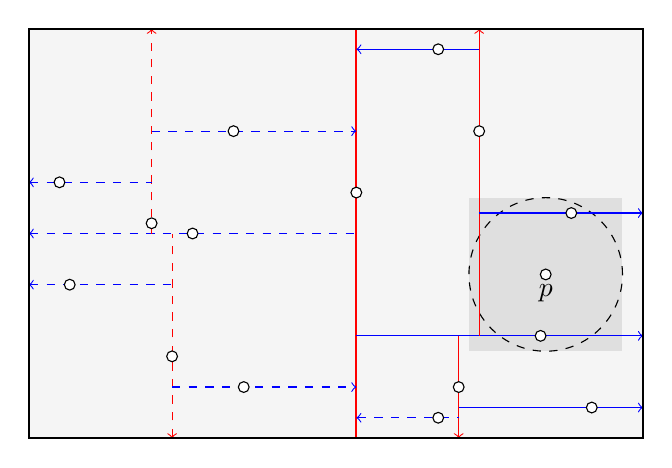
\begin{tikzpicture}[scale=1.3]
		\fill[lightgray!15] (0,0) rectangle (6,4);
		\fill[lightgray!50] (4.3,0.85) rectangle (5.8,2.35);
		\draw[dashed](5.05,1.6) circle(0.75);
		\fill[white,draw=black] (5.05,1.6) circle(1.5pt);
		\node[below] at (5.05,1.6) {$\tiny p$};
		
		\draw [red,thick](3.2,0) -- (3.2,4);
		\fill[white,draw=black] (3.2,2.4) circle (1.5pt);
		\draw [blue,->](3.2,1) -- (6,1);
		\fill[white,draw=black] (5,1) circle (1.5pt);
		\draw [red,<-](4.2,0) -- (4.2,1);
		\fill[white,draw=black] (4.2,0.5) circle (1.5pt);
		\draw [blue,<-,dashed](3.2,0.2) -- (4.2,0.2);
		\fill[white,draw=black] (4,0.2) circle (1.5pt);
		\draw [blue,->](4.2,0.3) -- (6,0.3);
		\fill[white,draw=black] (5.5,0.3) circle (1.5pt);
		\draw [red,->](4.4,1) -- (4.4,4);
		\fill[white,draw=black] (4.4,3) circle (1.5pt);
		\draw [blue,<-](3.2,3.8) -- (4.4,3.8);
		\fill[white,draw=black] (4,3.8) circle (1.5pt);
		\draw [blue,->](4.4,2.2) -- (6,2.2);
		\fill[white,draw=black] (5.3,2.2) circle (1.5pt);
		\draw [blue,<-,dashed](0,2) -- (3.2,2);
		\fill[white,draw=black] (1.6,2) circle (1.5pt);
		\draw [red,->,dashed](1.2,2) -- (1.2,4);
		\fill[white,draw=black] (1.2,2.1) circle (1.5pt);
		\draw [blue,->,dashed](1.2,3) -- (3.2,3);
		\fill[white,draw=black] (2,3) circle (1.5pt);
		\draw [blue,<-,dashed](0,2.5) -- (1.2,2.5);
		\fill[white,draw=black] (0.3,2.5) circle (1.5pt);
		\draw [red,<-,dashed](1.4,0) -- (1.4,2);
		\fill[white,draw=black] (1.4,0.8) circle (1.5pt);
		\draw [blue,->,dashed](1.4,0.5) -- (3.2,0.5);
		\fill[white,draw=black] (2.1,0.5) circle (1.5pt);
		\draw [blue,<-,dashed](0,1.5) -- (1.4,1.5);
		\fill[white,draw=black] (0.4,1.5) circle (1.5pt);
		\draw[thick] (0,0) rectangle (6,4);
		\end{tikzpicture}
	\end{center}
	\label{fig:kdrs}
\end{figure}